\documentclass{standalone}
\usepackage{tikz}
\usetikzlibrary{patterns, positioning}


\begin{document}
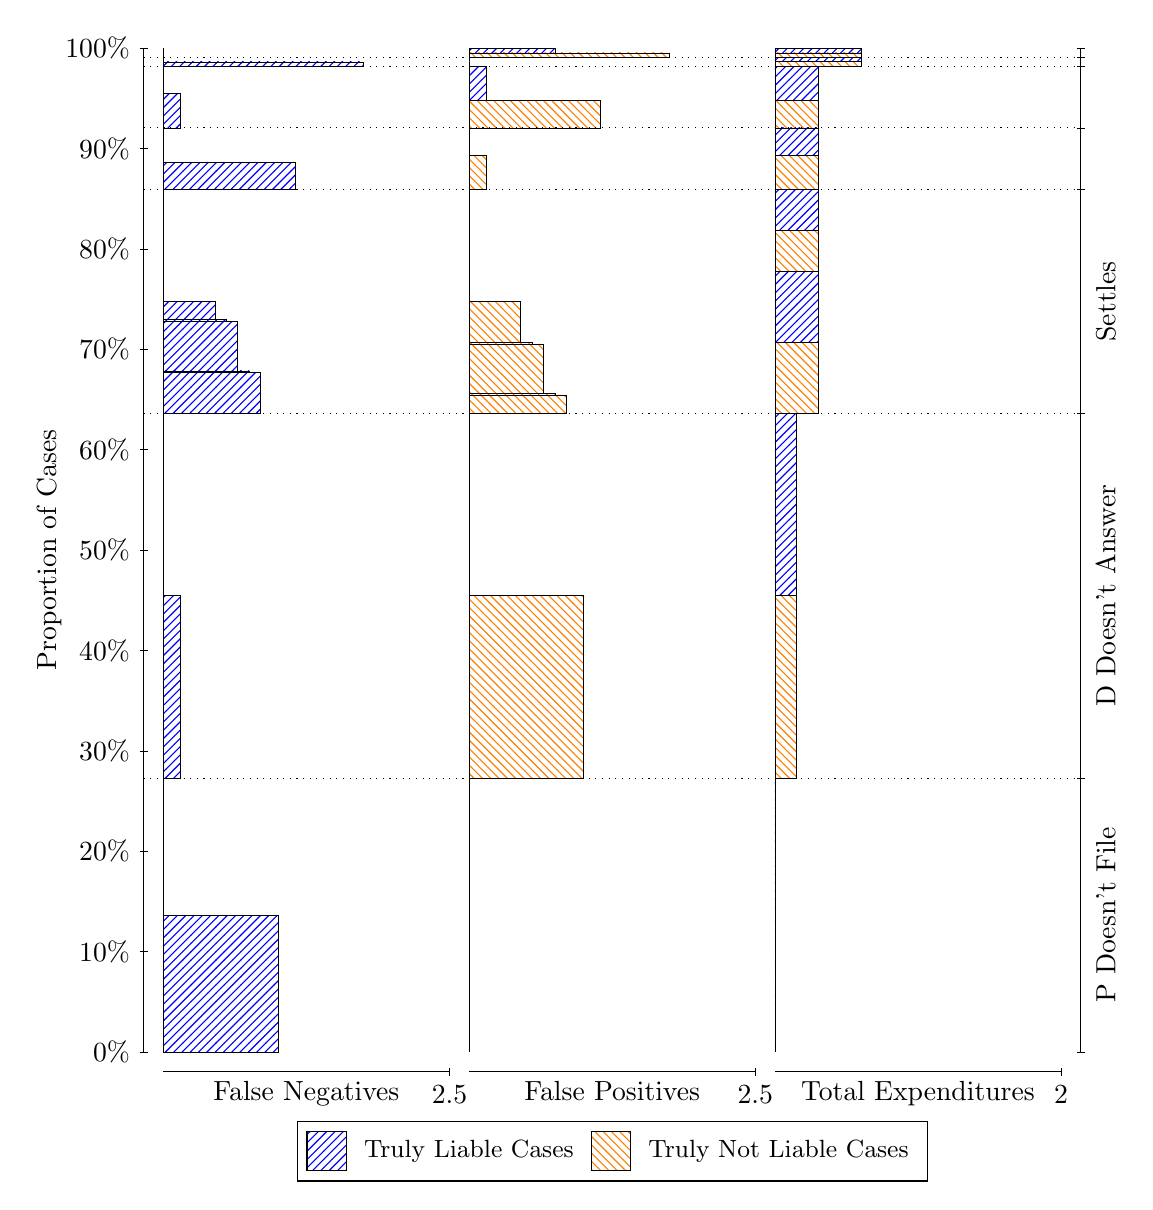
\begin{tikzpicture}
\draw[black, very thin] (1.5,1.75) -- (1.5,14.5);
\node[rotate=90, text=black, anchor=center] at (0.3, 8.125) {Proportion of Cases};
\draw[black, very thin] (1.45,1.75) -- (1.55,1.75);
\node[text=black, anchor=east] at (1.45, 1.75) {0\%};
\draw[black, very thin] (1.45,3.025) -- (1.55,3.025);
\node[text=black, anchor=east] at (1.45, 3.025) {10\%};
\draw[black, very thin] (1.45,4.3) -- (1.55,4.3);
\node[text=black, anchor=east] at (1.45, 4.3) {20\%};
\draw[black, very thin] (1.45,5.575) -- (1.55,5.575);
\node[text=black, anchor=east] at (1.45, 5.575) {30\%};
\draw[black, very thin] (1.45,6.85) -- (1.55,6.85);
\node[text=black, anchor=east] at (1.45, 6.85) {40\%};
\draw[black, very thin] (1.45,8.125) -- (1.55,8.125);
\node[text=black, anchor=east] at (1.45, 8.125) {50\%};
\draw[black, very thin] (1.45,9.4) -- (1.55,9.4);
\node[text=black, anchor=east] at (1.45, 9.4) {60\%};
\draw[black, very thin] (1.45,10.675) -- (1.55,10.675);
\node[text=black, anchor=east] at (1.45, 10.675) {70\%};
\draw[black, very thin] (1.45,11.95) -- (1.55,11.95);
\node[text=black, anchor=east] at (1.45, 11.95) {80\%};
\draw[black, very thin] (1.45,13.225) -- (1.55,13.225);
\node[text=black, anchor=east] at (1.45, 13.225) {90\%};
\draw[black, very thin] (1.45,14.5) -- (1.55,14.5);
\node[text=black, anchor=east] at (1.45, 14.5) {100\%};

\draw[black, very thin] (13.4,1.75) -- (13.4,14.5);
\draw[black, very thin] (13.35,1.75) -- (13.45,1.75);
\node[anchor=west] at (13.35, 1.75) {};
\draw[black, very thin] (13.35,5.2273) -- (13.45,5.2273);
\node[anchor=west] at (13.35, 5.2273) {};
\draw[black, very thin] (13.35,9.8636) -- (13.45,9.8636);
\node[anchor=west] at (13.35, 9.8636) {};
\draw[black, very thin] (13.35,12.703) -- (13.45,12.703);
\node[anchor=west] at (13.35, 12.703) {};
\draw[black, very thin] (13.35,13.487) -- (13.45,13.487);
\node[anchor=west] at (13.35, 13.487) {};
\draw[black, very thin] (13.35,14.27) -- (13.45,14.27);
\node[anchor=west] at (13.35, 14.27) {};
\draw[black, very thin] (13.35,14.385) -- (13.45,14.385);
\node[anchor=west] at (13.35, 14.385) {};
\draw[black, very thin] (13.35,14.5) -- (13.45,14.5);
\node[anchor=west] at (13.35, 14.5) {};

\draw[black, very thin, pattern color=blue, pattern=north east lines] (1.75,1.75) rectangle (3.2033,3.4886);
\draw[black, very thin, pattern color=orange, pattern=north west lines] (1.75,3.4886) rectangle (1.75,5.2273);
\draw[black, very thin, pattern color=blue, pattern=north east lines] (1.75,5.2273) rectangle (1.968,7.5455);
\draw[black, very thin, pattern color=orange, pattern=north west lines] (1.75,7.5455) rectangle (1.75,9.8636);
\draw[black, very thin, pattern color=blue, pattern=north east lines] (1.75,9.8636) rectangle (2.9853,10.378);
\draw[black, very thin, pattern color=blue, pattern=north east lines] (1.75,10.378) rectangle (2.84,10.401);
\draw[black, very thin, pattern color=blue, pattern=north east lines] (1.75,10.401) rectangle (2.6947,11.03);
\draw[black, very thin, pattern color=blue, pattern=north east lines] (1.75,11.03) rectangle (2.5493,11.049);
\draw[black, very thin, pattern color=blue, pattern=north east lines] (1.75,11.049) rectangle (2.404,11.283);
\draw[black, very thin, pattern color=orange, pattern=north west lines] (1.75,11.283) rectangle (1.75,12.703);
\draw[black, very thin, pattern color=blue, pattern=north east lines] (1.75,12.703) rectangle (3.4213,13.05);
\draw[black, very thin, pattern color=orange, pattern=north west lines] (1.75,13.05) rectangle (1.75,13.487);
\draw[black, very thin, pattern color=blue, pattern=north east lines] (1.75,13.487) rectangle (1.968,13.924);
\draw[black, very thin, pattern color=orange, pattern=north west lines] (1.75,13.924) rectangle (1.75,14.27);
\draw[black, very thin, pattern color=blue, pattern=north east lines] (1.75,14.27) rectangle (4.2933,14.323);
\draw[black, very thin, pattern color=orange, pattern=north west lines] (1.75,14.323) rectangle (1.75,14.385);
\draw[black, very thin, pattern color=orange, pattern=north west lines] (1.75,14.385) rectangle (1.75,14.438);
\draw[black, very thin, pattern color=blue, pattern=north east lines] (1.75,14.438) rectangle (1.75,14.5);
\draw[black, very thin, pattern color=orange, pattern=north west lines] (5.6333,1.75) rectangle (5.6333,3.4886);
\draw[black, very thin, pattern color=blue, pattern=north east lines] (5.6333,3.4886) rectangle (5.6333,5.2273);
\draw[black, very thin, pattern color=orange, pattern=north west lines] (5.6333,5.2273) rectangle (7.0867,7.5455);
\draw[black, very thin, pattern color=blue, pattern=north east lines] (5.6333,7.5455) rectangle (5.6333,9.8636);
\draw[black, very thin, pattern color=orange, pattern=north west lines] (5.6333,9.8636) rectangle (6.8687,10.089);
\draw[black, very thin, pattern color=orange, pattern=north west lines] (5.6333,10.089) rectangle (6.7233,10.112);
\draw[black, very thin, pattern color=orange, pattern=north west lines] (5.6333,10.112) rectangle (6.578,10.74);
\draw[black, very thin, pattern color=orange, pattern=north west lines] (5.6333,10.74) rectangle (6.4327,10.76);
\draw[black, very thin, pattern color=orange, pattern=north west lines] (5.6333,10.76) rectangle (6.2873,11.283);
\draw[black, very thin, pattern color=blue, pattern=north east lines] (5.6333,11.283) rectangle (5.6333,12.703);
\draw[black, very thin, pattern color=orange, pattern=north west lines] (5.6333,12.703) rectangle (5.8513,13.14);
\draw[black, very thin, pattern color=blue, pattern=north east lines] (5.6333,13.14) rectangle (5.6333,13.487);
\draw[black, very thin, pattern color=orange, pattern=north west lines] (5.6333,13.487) rectangle (7.3047,13.833);
\draw[black, very thin, pattern color=blue, pattern=north east lines] (5.6333,13.833) rectangle (5.8513,14.27);
\draw[black, very thin, pattern color=orange, pattern=north west lines] (5.6333,14.27) rectangle (5.6333,14.332);
\draw[black, very thin, pattern color=blue, pattern=north east lines] (5.6333,14.332) rectangle (5.6333,14.385);
\draw[black, very thin, pattern color=orange, pattern=north west lines] (5.6333,14.385) rectangle (8.1767,14.438);
\draw[black, very thin, pattern color=blue, pattern=north east lines] (5.6333,14.438) rectangle (6.7233,14.5);
\draw[black, very thin, pattern color=orange, pattern=north west lines] (9.5167,1.75) rectangle (9.5167,3.4886);
\draw[black, very thin, pattern color=blue, pattern=north east lines] (9.5167,3.4886) rectangle (9.5167,5.2273);
\draw[black, very thin, pattern color=orange, pattern=north west lines] (9.5167,5.2273) rectangle (9.7892,7.5455);
\draw[black, very thin, pattern color=blue, pattern=north east lines] (9.5167,7.5455) rectangle (9.7892,9.8636);
\draw[black, very thin, pattern color=orange, pattern=north west lines] (9.5167,9.8636) rectangle (10.062,10.76);
\draw[black, very thin, pattern color=blue, pattern=north east lines] (9.5167,10.76) rectangle (10.062,11.665);
\draw[black, very thin, pattern color=orange, pattern=north west lines] (9.5167,11.665) rectangle (10.062,12.188);
\draw[black, very thin, pattern color=blue, pattern=north east lines] (9.5167,12.188) rectangle (10.062,12.703);
\draw[black, very thin, pattern color=orange, pattern=north west lines] (9.5167,12.703) rectangle (10.062,13.14);
\draw[black, very thin, pattern color=blue, pattern=north east lines] (9.5167,13.14) rectangle (10.062,13.487);
\draw[black, very thin, pattern color=orange, pattern=north west lines] (9.5167,13.487) rectangle (10.062,13.833);
\draw[black, very thin, pattern color=blue, pattern=north east lines] (9.5167,13.833) rectangle (10.062,14.27);
\draw[black, very thin, pattern color=orange, pattern=north west lines] (9.5167,14.27) rectangle (10.607,14.332);
\draw[black, very thin, pattern color=blue, pattern=north east lines] (9.5167,14.332) rectangle (10.607,14.385);
\draw[black, very thin, pattern color=orange, pattern=north west lines] (9.5167,14.385) rectangle (10.607,14.438);
\draw[black, very thin, pattern color=blue, pattern=north east lines] (9.5167,14.438) rectangle (10.607,14.5);
\draw[black, dotted] (1.5,5.2273) -- (13.4,5.2273);
\draw[black, dotted] (1.5,9.8636) -- (13.4,9.8636);
\draw[black, dotted] (1.5,12.703) -- (13.4,12.703);
\draw[black, dotted] (1.5,13.487) -- (13.4,13.487);
\draw[black, dotted] (1.5,14.27) -- (13.4,14.27);
\draw[black, dotted] (1.5,14.385) -- (13.4,14.385);
\draw[black, very thin] (1.75,1.5) -- (5.3833,1.5);
\node[text=black, anchor=north] at (3.5667, 1.5) {False Negatives};
\draw[black, very thin] (5.3833,1.45) -- (5.3833,1.55);
\node[text=black, anchor=north] at (5.3833, 1.45) {2.5};

\draw[black, very thin] (5.6333,1.5) -- (9.2667,1.5);
\node[text=black, anchor=north] at (7.45, 1.5) {False Positives};
\draw[black, very thin] (9.2667,1.45) -- (9.2667,1.55);
\node[text=black, anchor=north] at (9.2667, 1.45) {2.5};

\draw[black, very thin] (9.5167,1.5) -- (13.15,1.5);
\node[text=black, anchor=north] at (11.333, 1.5) {Total Expenditures};
\draw[black, very thin] (13.15,1.45) -- (13.15,1.55);
\node[text=black, anchor=north] at (13.15, 1.45) {2};

\node[text=black, centered, rotate=90] at (13.72, 3.4886) {P Doesn't File};
\node[text=black, centered, rotate=90] at (13.72, 7.5455) {D Doesn't Answer};
\node[text=black, centered, rotate=90] at (13.72, 11.283) {Settles};





\draw (7.449999999999999,1.5) node[draw=none] (baseCoordinate) {};
\begin{scope}[align=center]
        \matrix[scale=0.5, draw=black, below=0.5cm of baseCoordinate, nodes={draw}, column sep=0.1cm]{
            \node[rectangle, draw, minimum width=0.5cm, minimum height=0.5cm, pattern color=blue, pattern=north east lines] {}; &
            \node[draw=none, font=\small, text=black] (B) {Truly Liable Cases}; &
            \node[rectangle, draw, minimum width=0.5cm, minimum height=0.5cm, pattern color=orange, pattern=north west lines] {}; &
            \node[draw=none, font=\small, text=black] (B) {Truly Not Liable Cases}; \\
            };
\end{scope}

\end{tikzpicture}
\end{document}